\begin{frame}{Entanglement Entropy Area Law} 
\vskip-1.5cm
Ground states of gapped quantum Hamiltonians satisfy an area law: 
$$
S_V \lesssim d \cdot (\partial V) - \gamma
$$

$\gamma$ is universal and detects presence of topological order

In 1D:

\begin{columns}[T]
    \begin{column}[T]{.33\textwidth}
        \begin{figure}[h]
            %\captionsetup{justification=right}
            \centering
            $$S(x) \lesssim d $$
            \scalebox{0.45}{
             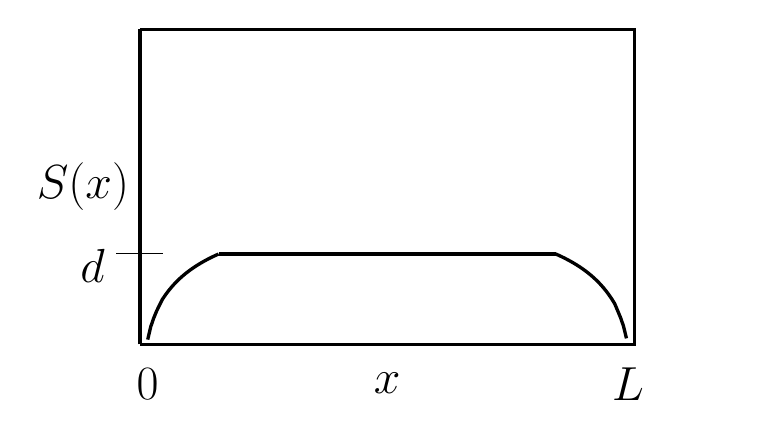
\begin{tikzpicture}[domain=0.1:6.18]
      \draw[very thick] (0, 0) -- (0,4) node[left, midway] {\LARGE $S(x)$} ;
     \node[] at (7.5, 2) {$$};
      \node[] at (3.14, -0.5){\LARGE $x$};
      \node[] at (-0.6, 1){\LARGE $d$};
      \draw[] (-0.3, 1.15) -- (0.3, 1.15);
       \node[] at (0.1, -0.5){\LARGE $0$};
       \node[] at (6.2, -0.5){\LARGE $L$};
      % \draw[thick] (0, 3.05) -- (3.14, 3.05);
      \draw[very thick] (0, 4)-- (6.28,4) -- (6.28, 0) -- (0, 0);
      \draw[color=black, very thick, domain=0.1:1] plot (\x,{1.5+1/3*log2(sin(\x/2 r))}) node[right] {};
	\draw[color=black, very thick, domain=1:5.28] plot (\x,{1.5+1/3*log2(sin(1/2 r))}) node[right] {};
	\draw[color=black, very thick, domain=5.28:6.18] plot (\x,{1.5+1/3*log2(sin(\x/2 r))}) node[right] {};
\end{tikzpicture}
            }
            \caption{Gapped ground state}
        \end{figure}
    \end{column}
    \begin{column}[T]{.33\textwidth}
            \begin{figure}[h]
            %\captionsetup{justification=right}
            \centering
            $$S(x) \lesssim c \log{x}$$
            \scalebox{0.45}{
             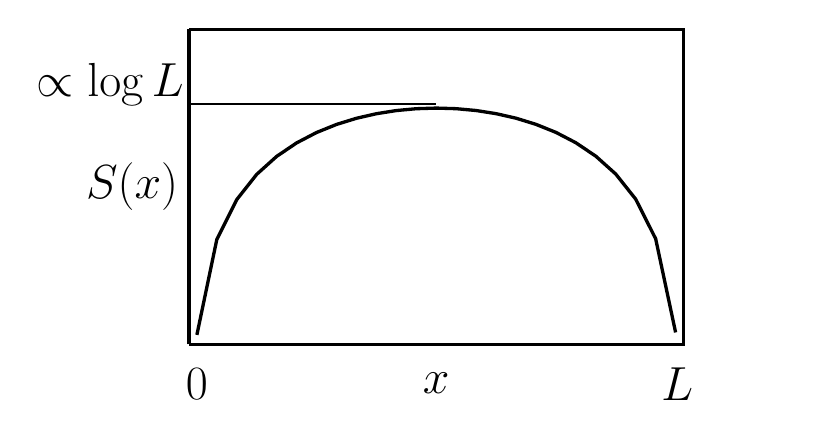
\begin{tikzpicture}[domain=0.1:6.18]
      \draw[very thick] (0, 0) -- (0,4) node[left, midway] {\LARGE $S(x)$} ;
       \node[] at (7.5, 2) {$$};
      \node[] at (3.14, -0.5){\LARGE $x$};
       \node[] at (-1, 3.3){\LARGE $\propto \log{L}$};
       \node[] at (0.1, -0.5){\LARGE $0$};
       \node[] at (6.2, -0.5){\LARGE $L$};
       \draw[thick] (0, 3.05) -- (3.14, 3.05);
      \draw[very thick] (0, 4)-- (6.28,4) -- (6.28, 0) -- (0, 0);
            \draw[color=black, very thick] plot (\x,{3+2/3*log2(sin(\x/2 r))}) node[right] {};
  \end{tikzpicture}
            }
            \caption{Gapless ground state}
        \end{figure}
    \end{column}
    \begin{column}[T]{.33\textwidth}
            \begin{figure}[h]
            %\captionsetup{justification=right}
            \centering
            $$S(x) \propto x $$
            \scalebox{0.45}{
             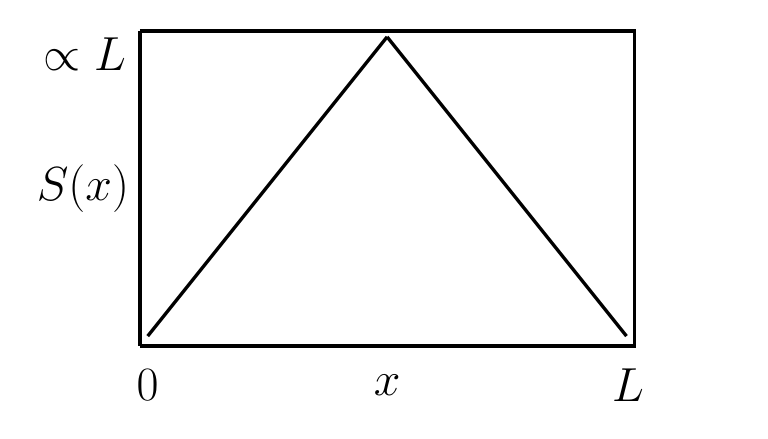
\begin{tikzpicture}[domain=0.1:6.18]
      \draw[very thick] (0, 0) -- (0,4) node[left, midway] {\LARGE $S(x)$} ;
       \node[] at (7.5, 2) {$$};
      \node[] at (3.14, -0.5){\LARGE $x$};
      \node[] at (0.1, -0.5){\LARGE $0$};
      \node[] at (6.2, -0.5){\LARGE $L$};
      \node[] at (-0.7, 3.7){\LARGE $\propto L$};
      \draw[very thick] (0, 4)-- (6.28,4) -- (6.28, 0) -- (0, 0);
      \draw[color=black, very thick, domain=0.1:3.14] plot (\x,{1.25*\x}) node[right] {};
      \draw[color=black, very thick, domain=3.14:6.18] plot (\x,{1.25*(6.28 - \x)}) node[right] {};
  \end{tikzpicture}
            }
            \caption{Generic State}
        \end{figure}
    \end{column}
\end{columns}
\end{frame}
    